\section{TẬP HỢP VÀ CÁC PHÉP TOÁN TRÊN TẬP HỢP}

\subsection{TÓM TẮT LÝ THUYẾT}

\subsubsection{Các khái niệm về tập hợp}
\begin{enumerate}[\iconMT]
	\item \indam{Tập hợp}
	\begin{enumerate}[\faPencilSquareO]
		\item Khi muốn mô tả các đối tượng (phần tử) có chung một tính chất thì ta xây dựng khái niệm tập hợp.
		\begin{boxkn}
		\begin{itemize}
			\item  Người ta thường dùng chữ cái in hoa $A$, $B$, $\cdots$ để kí hiệu tập hợp.
			\item  Để chỉ $a$ thuộc tập hợp $A$, ta viết $a \in A$; để chỉ $a$ không thuộc tập hợp $A$, ta viết $a \notin A$.
		\end{itemize}
		\end{boxkn}
		\item Cách xác định tập hợp: 
		\begin{boxkn}
		\begin{itemize}
			\item  Liệt kê các phần tử: viết các phần tử của tập hợp trong hai dấu móc $\left\{...\right\}$.
			\item  Chỉ ra tính chất đăc trưng cho các phần tử của tập hợp.
		\end{itemize}
		\end{boxkn}
		\item Tập rỗng: là tập hợp không chứa phần tử nào, kí hiệu $\varnothing $.
	\end{enumerate}	
\end{enumerate}
Cho hai tập hợp $A$ và $B$
\begin{enumerate}[\iconMT]
\item \indam{Tập hợp con:}  Nếu mọi phần tử của $A$ đều nằm trong $B$ thì ta nói tập $A$ là con của tập $B$, nghĩa là $$A\subset B\Leftrightarrow (\forall x\colon x \in A\Rightarrow x\in B)$$
\begin{tcolorbox}[colframe=cyan,colback=white,boxrule=0.2mm]
	\immini{\begin{itemize}
			\item  Các tính chất:
			\begin{listEX}[1]
				\item [\ding{172}] $A\subset A,\forall A$.
				\item [\ding{173}] $\varnothing \subset A,\forall A$.
				\item [\ding{174}] $A\subset B$, và $B\subset C$ suy ra $A\subset C$.
			\end{listEX}
			\item  Nếu $A$ không phải tập con của $B$ thì ta kí hiệu $A\not\subset B$.
			\item Nếu $A \subset B$ hoặc $B \subset A$ thì ta nói $A$ và $B$ có quan hệ bao hàm.
	\end{itemize}}{
		\begin{tikzpicture}[smooth,font=\footnotesize,scale=1]
			\def\miena{(0,0) to[bend left=90] (2,2) to[bend left=90] (0,0)}
			\def\mienb{(0.5,0.5) to[bend left=90] (1.5,1.75) to[bend left=90] (0.5,0.5)}
			\draw[pattern=dots] \miena;
			\draw[fill=white] \mienb
			(1,-0.7) node{Biểu đồ Ven minh họa $A \subset B$}
			(1,1.2) node{$A$}
			(0.5,0.1) node{$B$};
	\end{tikzpicture}}
\end{tcolorbox}
\item \indam{Tập hợp bằng nhau:} $A=B\Leftrightarrow A\subset B$ và $B\subset A\Leftrightarrow (\forall x \colon x\in A\Leftrightarrow x\in B)$.
\end{enumerate}
\subsubsection {Các tập hợp số}
\begin{tcolorbox}[colframe=cyan,colback=white,boxrule=0.2mm]
	\begin{listEX}[3]
		\item [\ding{172}] Tập số tự nhiên $\mathbb{N}$.
		\item [\ding{173}] Tập số nguyên $\mathbb{Z}$.
		\item [\ding{174}] Tập số hữu tỉ $\mathbb{Q}$.
		\item [\ding{175}] Tập số vô tỉ $\mathbb{I}$.
		\item [\ding{176}] Tập số thực $\mathbb{R}$.
		\item [\ding{177}] Tập $\mathbb{N^*}$ ta bỏ số $0$.
	\end{listEX}
\end{tcolorbox}	
	\begin{enumerate}[\iconMT]
\item \indamm{Mối quan hệ giữa các tập hợp số}
\begin{listEX}[2]
	\item [\ding{172}] $\mathbb{N} \subset \mathbb{Z} \subset \mathbb{Q} \subset \mathbb{R}$.
	\item [\ding{173}] $\mathbb{Q} \cup \mathbb{I}=\mathbb{R}$.
\end{listEX}
\item \indam{Một số tập con của tập hợp số thực}

\begin{tcolorbox}[colframe=orange,colback=white,boxrule=0.2mm]
	\begin{listEX}[2]
		\item [\ding{172}] Khoảng $\left(a;b\right)=\left\{\left. x\in \mathbb{R}\right|a<x<b\right\}$.\\
		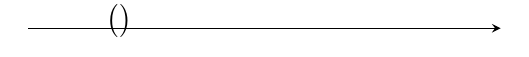
\begin{tikzpicture}[>=stealth]
			\draw[->](-1,0)->(5,0);
			\IntervalLR{-1}{1/2}
			\def\skipInterval{0.5cm}%Khoảng cách đặt nhãn
			\IntervalGRF{}{}{\big(}{a}%Gạch xọc phải qua trái
			\IntervalLR{4}{4.8}
			\def\skipInterval{0.5cm}%Khoảng cách đặt nhãn
			\IntervalGRF{\big)}{b}{}{}%Gạch xọc phải qua trái
		\end{tikzpicture}	
		\item [\ding{173}] Đoạn $\left[a;b\right]=\left\{\left. x\in \mathbb{R}\right|a\le x\le b\right\}$.\\
		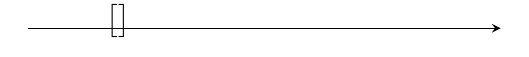
\begin{tikzpicture}[>=stealth]
			\draw[->](-1,0)->(5,0);
			\IntervalLR{-1}{1/2}
			\def\skipInterval{0.5cm}%Khoảng cách đặt nhãn
			\IntervalGRF{}{}{\big[}{a}%Gạch xọc phải qua trái
			\IntervalLR{4}{4.8}
			\def\skipInterval{0.5cm}%Khoảng cách đặt nhãn
			\IntervalGRF{\big]}{b}{}{}%Gạch xọc phải qua trái
		\end{tikzpicture}
		\item [\ding{174}] Khoảng $\left(a;+\infty \right)=\left\{\left. x\in \mathbb{R}\right|x>a\right\}$.\\
		\begin{tikzpicture}[>=stealth]
			\draw[->](-1,0)--(5,0)node[below]{$+\infty$};
			\IntervalLR{-1}{1/2}
			\def\skipInterval{0.5cm}%Khoảng cách đặt nhãn
			\IntervalGRF{}{}{\big(}{a}%Gạch xọc phải qua trái
			\IntervalLR{4}{4.8}
			\def\skipInterval{0.5cm}%Khoảng cách đặt nhãn
			%\IntervalGRF{\big]}{b}{}{}%Gạch xọc phải qua trái
		\end{tikzpicture}
		\item [\ding{175}] Nửa khoảng $\left[a;+\infty \right)=\left\{\left. x\in \mathbb{R}\right|x\ge a\right\}$.\\
		\begin{tikzpicture}[>=stealth]
			\draw[->](-1,0)->(5,0)node[below]{$+\infty$};
			\IntervalLR{-1}{1/2}
			\def\skipInterval{0.5cm}%Khoảng cách đặt nhãn
			\IntervalGRF{}{}{\big[}{a}%Gạch xọc phải qua trái
			\IntervalLR{4}{4.8}
			\def\skipInterval{0.5cm}%Khoảng cách đặt nhãn
			%\IntervalGRF{\big]}{b}{}{}%Gạch xọc phải qua trái
		\end{tikzpicture}
		\item [\ding{176}] Khoảng $\left(-\infty;b\right)=\left\{\left. x\in \mathbb{R}\right|x<b\right\}$.\\
		\begin{tikzpicture}[>=stealth]
			\draw[->](-1,0)node[below]{$-\infty$}--(5,0);
			\IntervalLR{-1}{1/2}
			\def\skipInterval{0.5cm}%Khoảng cách đặt nhãn
			%\IntervalGRF{}{}{\big[}{a}%Gạch xọc phải qua trái
			\IntervalLR{3}{4.8}
			\def\skipInterval{0.5cm}%Khoảng cách đặt nhãn
			\IntervalGRF{\big)}{b}{}{}%Gạch xọc phải qua trái
		\end{tikzpicture}
		\item [\ding{177}] Nửa khoảng $\left(-\infty;b\right]=\left\{\left. x\in \mathbb{R}\right|x\le b\right\}$.\\
		\begin{tikzpicture}[>=stealth]
			\draw[->](-1,0)node[below]{$-\infty$}->(5,0);
			\IntervalLR{-1}{1/2}
			\def\skipInterval{0.5cm}%Khoảng cách đặt nhãn
			%\IntervalGRF{}{}{\big[}{a}%Gạch xọc phải qua trái
			\IntervalLR{3}{4.8}
			\def\skipInterval{0.5cm}%Khoảng cách đặt nhãn
			\IntervalGRF{\big]}{b}{}{}%Gạch xọc phải qua trái
		\end{tikzpicture}
		\item [\ding{178}] Nửa khoảng $\left[a;b\right)=\left\{\left. x\in \mathbb{R}\right|a\le x<b\right\}$.\\
		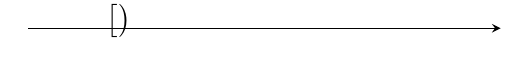
\begin{tikzpicture}[>=stealth]
			\draw[->](-1,0)->(5,0);
			\IntervalLR{-1}{1/2}
			\def\skipInterval{0.5cm}%Khoảng cách đặt nhãn
			\IntervalGRF{}{}{\big[}{a}%Gạch xọc phải qua trái
			\IntervalLR{4}{4.8}
			\def\skipInterval{0.5cm}%Khoảng cách đặt nhãn
			\IntervalGRF{\big)}{b}{}{}%Gạch xọc phải qua trái
		\end{tikzpicture}
		\item [\ding{179}] Nửa khoảng $\left(a;b\right]=\left\{\left. x\in \mathbb{R}\right|a<x\le b\right\}$.\\
		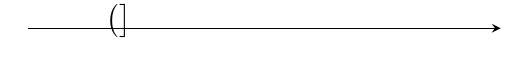
\begin{tikzpicture}[>=stealth]
			\draw[->](-1,0)->(5,0);
			\IntervalLR{-1}{1/2}
			\def\skipInterval{0.5cm}%Khoảng cách đặt nhãn
			\IntervalGRF{}{}{\big(}{a}%Gạch xọc phải qua trái
			\IntervalLR{4}{4.8}
			\def\skipInterval{0.5cm}%Khoảng cách đặt nhãn
			\IntervalGRF{\big]}{b}{}{}%Gạch xọc phải qua trái
		\end{tikzpicture}
	\end{listEX}
\end{tcolorbox}
\end{enumerate}

\subsubsection{Các phép toán trên tập hợp}
\begin{enumerate}[\iconMT]
	\item \indamm{Hợp của hai tập hợp}
	\immini{\begin{itemize}
			\item  $A\cup B=\{x|x\in A$ hoặc $x\in B \} $.
			\item  Ghi nhớ: Gom hết phần tử của cả hai tập, các phần tử trùng nhau thì ta ghi 1 lần.
	\end{itemize}}{\vspace{-1cm}
		\begin{tikzpicture}[smooth,font=\footnotesize,scale=0.8]
			\draw[pattern=north east lines,pattern color=orange]
			(0,0) to[bend left=90] (2,2) to[bend left=90] (0,0)
			(1,0) to[bend left=90] (3,2) to[bend left=90] (1,0)
			(1,-0.7) node{Biểu đồ Ven minh họa $A \cup B$}
			(0.5,1) node{$A$}
			(2.6,0.9) node{$B$};
	\end{tikzpicture}}
\item \indamm{Giao của hai tập hợp}
\immini{\begin{itemize}
		\item  $A\cap B= \{x|x\in A$ và $x\in B \}$.
		\item  Ghi nhớ: Lấy phần chung của 2 tập hợp.
\end{itemize}}{\vspace{-1cm}
	\begin{tikzpicture}[smooth,font=\footnotesize,scale=0.8]
		\def\miena{(0,0) to[bend left=90] (2,2) to[bend left=90] (0,0)}
		\def\mienb{(1,0) to[bend left=90] (3,2) to[bend left=90] (1,0)}
		\begin{scope}
			\clip \miena;
			\draw[pattern=north east lines,pattern color=orange] \mienb;
		\end{scope}
		\draw \miena \mienb
		(1,-0.7) node{Biểu đồ Ven minh họa $A \cap B$}
		(0.5,1) node{$A$}
		(2.6,0.9) node{$B$};
\end{tikzpicture}}
\item \indamm{Hiệu của hai tập hợp, phần bù của tập con}
\begin{itemize}
	\item  $A\backslash B= \{x|x\in A$ và $x\notin B \} $.
	\item  Ghi nhớ: Lấy phần riêng (thuộc A mà không thuộc B)
	\item Đặc biệt: Nếu $B\subset A$ thì $A\backslash B$ được kí hiệu là \fbox{$C_AB$} (gọi là phần bù của $B$ trong $A$).
\end{itemize}
\hspace*{2cm}
\begin{tikzpicture}[smooth,font=\footnotesize,scale=1]
	\def\miena{(0,0) to[bend left=90] (2,2) to[bend left=90] (0,0)}
	\def\mienb{(1,0) to[bend left=90] (3,2) to[bend left=90] (1,0)}
	\fill[pattern=north east lines,pattern color=orange] \miena;
	\draw[fill=white] \mienb
	(1,-0.7) node{Biểu đồ Ven minh họa $A \backslash B$}
	(0.5,1) node{$A$}
	(2.6,0.9) node{$B$};
	\draw \miena ;
\end{tikzpicture}
\hspace{3cm}
\begin{tikzpicture}[smooth,font=\footnotesize,scale=1]
	\def\miena{(0,0) to[bend left=90] (2,2) to[bend left=90] (0,0)}
	\def\mienb{(0.5,0.5) to[bend left=90] (1.5,1.75) to[bend left=90] (0.5,0.5)}
	\draw[pattern=dots,pattern color=orange] \miena;
	\draw[fill=white] \mienb
	(1,-0.7) node{Biểu đồ Ven minh họa phần bù của $B$ trong $A$}
	(1,1.2) node{$B$}
	(0.5,0.1) node{$C_AB$}
	(2.3,0.8) node{$A$};
\end{tikzpicture}
\end{enumerate}